\XtoCBlock{Saturation}
\label{block:Saturation}
\begin{figure}[H]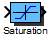
\includegraphics{Saturation}\end{figure} 

\begin{XtoCtabular}{Inports}
In & Input\tabularnewline
\hline
\end{XtoCtabular}


\begin{XtoCtabular}{Outports}
Out & Limited output\tabularnewline
\hline
\end{XtoCtabular}

\begin{XtoCtabular}{Mask Parameters}
max & Upper Limit\tabularnewline
\hline
min & Lower Limit\tabularnewline
\hline
\end{XtoCtabular}

\subsubsection*{Description:}
Saturation of output to adjustable upper and lower limit.

% include optional documentation file
\InputIfFileExists{\XcHomePath/Library/General/Doc/Saturation_Info.tex}{\vspace{1ex}}{}

\subsubsection*{Implementations:}
\begin{tabular}{l l}
\textbf{FiP8} & 8 Bit Fixed Point Implementation\tabularnewline
\textbf{FiP16} & 16 Bit Fixed Point Implementation\tabularnewline
\textbf{FiP32} & 32 Bit Fixed Point Implementation\tabularnewline
\textbf{Float32} & 32 Bit Floating Point Implementation\tabularnewline
\textbf{Float64} & 64 Bit Floating Point Implementation\tabularnewline
\end{tabular}

\XtoCImplementation{FiP8}
\index{Block ID!80}
\nopagebreak[0]
% Implementation details
\begin{tabular}{l l}
\textbf{Name} & FiP8 \tabularnewline
\textbf{ID} & 80 \tabularnewline
\textbf{Revision} & 1.0 \tabularnewline
\textbf{C filename} & Saturation\_FiP8.c \tabularnewline
\textbf{H filename} & Saturation\_FiP8.h \tabularnewline
\end{tabular}
\vspace{1ex}

8 Bit Fixed Point Implementation

\begin{XtoCtabular}{Controller Parameters}
max & Upper limit\tabularnewline
\hline
min & Lower limit\tabularnewline
\hline
\end{XtoCtabular}

% Implementation data structure
\XtoCDataStruct{Data Structure:}
\begin{lstlisting}
typedef struct {
     uint16        ID;
     int8          *In;
     int8          Out;
     int8          max;
     int8          min;
} SATURATION_FIP8;
\end{lstlisting}

\ifdefined \AddTestReports
\InputIfFileExists{\XcHomePath/Library/General/Doc/Test_Saturation_FiP8.tex}{}{}
\fi
\XtoCImplementation{FiP16}
\index{Block ID!81}
\nopagebreak[0]
% Implementation details
\begin{tabular}{l l}
\textbf{Name} & FiP16 \tabularnewline
\textbf{ID} & 81 \tabularnewline
\textbf{Revision} & 1.0 \tabularnewline
\textbf{C filename} & Saturation\_FiP16.c \tabularnewline
\textbf{H filename} & Saturation\_FiP16.h \tabularnewline
\end{tabular}
\vspace{1ex}

16 Bit Fixed Point Implementation

\begin{XtoCtabular}{Controller Parameters}
max & Upper limit\tabularnewline
\hline
min & Lower limit\tabularnewline
\hline
\end{XtoCtabular}

% Implementation data structure
\XtoCDataStruct{Data Structure:}
\begin{lstlisting}
typedef struct {
     uint16        ID;
     int16         *In;
     int16         Out;
     int16         max;
     int16         min;
} SATURATION_FIP16;
\end{lstlisting}

\ifdefined \AddTestReports
\InputIfFileExists{\XcHomePath/Library/General/Doc/Test_Saturation_FiP16.tex}{}{}
\fi
\XtoCImplementation{FiP32}
\index{Block ID!82}
\nopagebreak[0]
% Implementation details
\begin{tabular}{l l}
\textbf{Name} & FiP32 \tabularnewline
\textbf{ID} & 82 \tabularnewline
\textbf{Revision} & 1.0 \tabularnewline
\textbf{C filename} & Saturation\_FiP32.c \tabularnewline
\textbf{H filename} & Saturation\_FiP32.h \tabularnewline
\end{tabular}
\vspace{1ex}

32 Bit Fixed Point Implementation

\begin{XtoCtabular}{Controller Parameters}
max & Upper limit\tabularnewline
\hline
min & Lower limit\tabularnewline
\hline
\end{XtoCtabular}

% Implementation data structure
\XtoCDataStruct{Data Structure:}
\begin{lstlisting}
typedef struct {
     uint16        ID;
     int32         *In;
     int32         Out;
     int32         max;
     int32         min;
} SATURATION_FIP32;
\end{lstlisting}

\ifdefined \AddTestReports
\InputIfFileExists{\XcHomePath/Library/General/Doc/Test_Saturation_FiP32.tex}{}{}
\fi
\XtoCImplementation{Float32}
\index{Block ID!83}
\nopagebreak[0]
% Implementation details
\begin{tabular}{l l}
\textbf{Name} & Float32 \tabularnewline
\textbf{ID} & 83 \tabularnewline
\textbf{Revision} & 0.1 \tabularnewline
\textbf{C filename} & Saturation\_Float32.c \tabularnewline
\textbf{H filename} & Saturation\_Float32.h \tabularnewline
\end{tabular}
\vspace{1ex}

32 Bit Floating Point Implementation

\begin{XtoCtabular}{Controller Parameters}
max & Upper limit\tabularnewline
\hline
min & Lower limit\tabularnewline
\hline
\end{XtoCtabular}

% Implementation data structure
\XtoCDataStruct{Data Structure:}
\begin{lstlisting}
typedef struct {
     uint16        ID;
     float32       *In;
     float32       Out;
     float32       max;
     float32       min;
} SATURATION_FLOAT32;
\end{lstlisting}

\ifdefined \AddTestReports
\InputIfFileExists{\XcHomePath/Library/General/Doc/Test_Saturation_Float32.tex}{}{}
\fi
\XtoCImplementation{Float64}
\index{Block ID!84}
\nopagebreak[0]
% Implementation details
\begin{tabular}{l l}
\textbf{Name} & Float64 \tabularnewline
\textbf{ID} & 84 \tabularnewline
\textbf{Revision} & 0.1 \tabularnewline
\textbf{C filename} & Saturation\_Float64.c \tabularnewline
\textbf{H filename} & Saturation\_Float64.h \tabularnewline
\end{tabular}
\vspace{1ex}

64 Bit Floating Point Implementation

\begin{XtoCtabular}{Controller Parameters}
max & Upper limit\tabularnewline
\hline
min & Lower limit\tabularnewline
\hline
\end{XtoCtabular}

% Implementation data structure
\XtoCDataStruct{Data Structure:}
\begin{lstlisting}
typedef struct {
     uint16        ID;
     float64       *In;
     float64       Out;
     float64       max;
     float64       min;
} SATURATION_FLOAT64;
\end{lstlisting}

\ifdefined \AddTestReports
\InputIfFileExists{\XcHomePath/Library/General/Doc/Test_Saturation_Float64.tex}{}{}
\fi
